\makeatletter\let\ifGm@compatii\relax\makeatother
\documentclass[landscape]{beamer}
\usepackage[nofancy,notoday]{rcsinfo}
\usepackage{color}
\usepackage{amsmath}
\usepackage{moreverb}
\usepackage{multicol}
\usepackage{graphicx}
\usepackage{floatflt}
%
\renewcommand{\b}{\mathbf}
\newcommand{\T}{^{T}}
\newcommand{\cs}[1]{$_{\text{#1}}$}
\newcommand{\inv}{^{\mathrm -1}}
\newcommand{\cp}[1]{$^{\text{#1}}$}
\newcommand{\degsym}{\ensuremath{^\circ}}
\newcommand{\newframe}[2][]{\begin{frame}\frametitle{\hfill #2 \hfil}}

\parskip 2pt
%
% -----------------------------------------------------------------------------
%
\title{Summary of Full Forward Model}
\subtitle{wvs-063r2}
\author{Van Snyder}
\date{4 December 2007}
\titlegraphic{\includegraphics[width=1.0in]{eos_mls_logo_onpink}}

\begin{document}
\sloppy
%
% -----------------------------------------------------------------------------
%
\begin{frame}
 \titlepage
\end{frame}
%
% -----------------------------------------------------------------------------
%
\newframe{Overview of {\tt mlsl2} program loop structure}
The {\tt mlsl2} program has nine levels of loops:
\begin{itemize}
\item The Chunk loop -- this is in the tree walker
\item The Phase loop -- this is explicitly unrolled in the l2cf
\item The Newton iteration loop -- this is in the retriever
\item The forward model MAF loop -- this is in the retriever
\item The forward model configuration loop -- this is in the retriever
\end{itemize}

The remaining four levels of loops are in the forward models:

\begin{itemize}
\item The sideband loop
\item The pointing (not MIF!) loop
\item The frequency loop
\item The path loops -- sometimes array operations
\end{itemize}

This presentation is limited to the full forward model.  See JPL D-18130.

\end{frame}
%
% -----------------------------------------------------------------------------
%
\newframe{Overview of {\tt mlsl2} program loop structure}

{\hfill 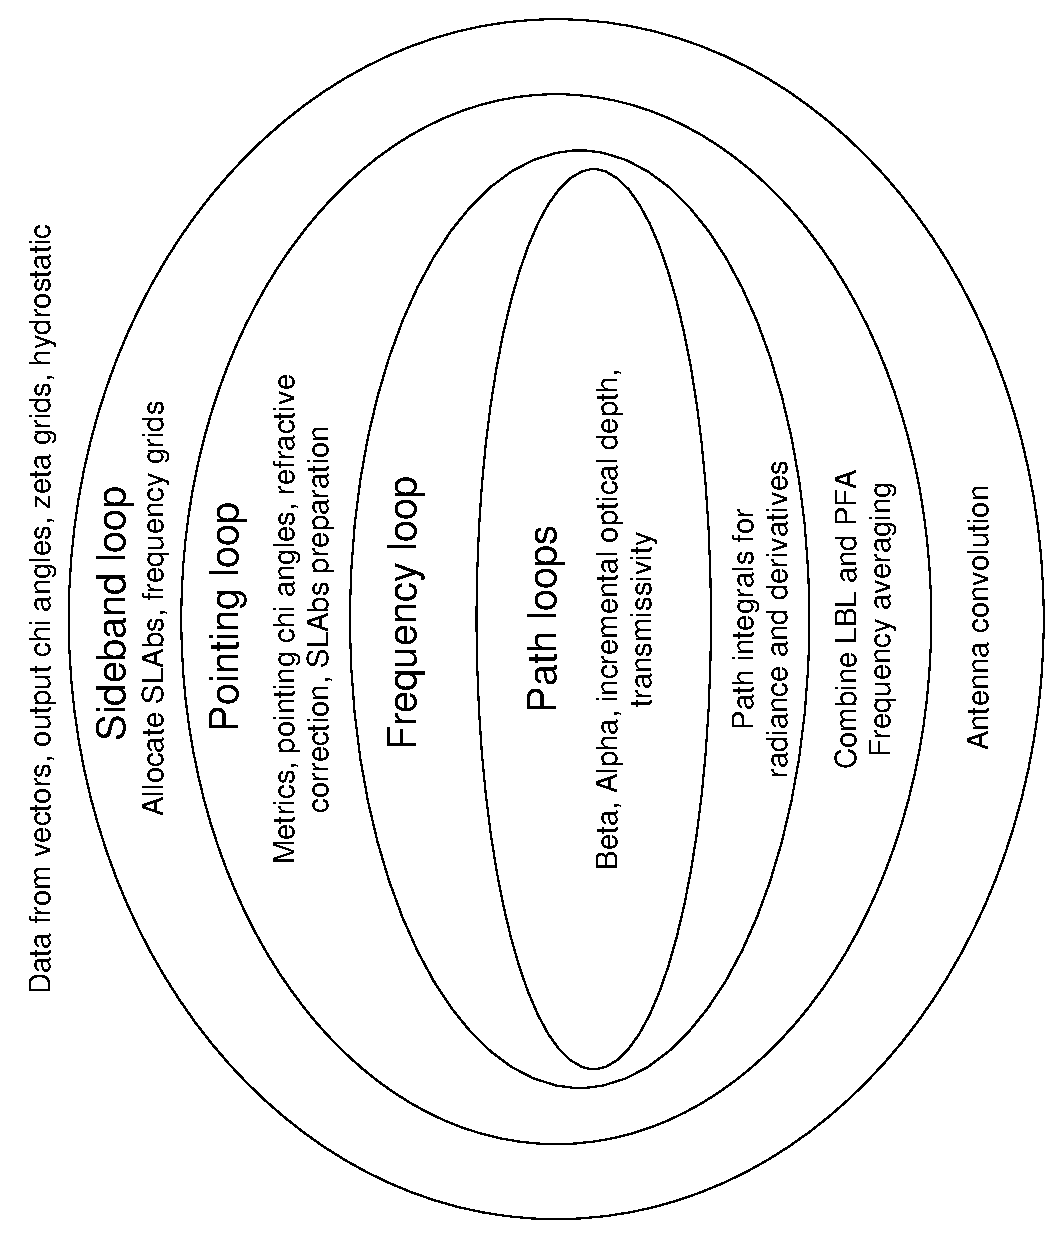
\includegraphics[scale=0.45,angle=270]{wvs-063-diag}
\hfill}

\end{frame}
%
% -----------------------------------------------------------------------------
%
\newframe{Data structures --- overview and arrays}

Most of the data structures in the full forward model are arrays.  In addition,
the {\tt Vector\_T}, {\tt VectorValue\_T}, {\tt ForwardModelConfig\_T} and {\tt
Grids\_T} structures are used. The {\tt Vector\_T} and {\tt VectorValue\_T}
structures are not further described here.

$\zeta \times \phi$ arrays, where $\phi$ is the horizontal representation basis
for temperature and $\zeta$ is the union of $\zeta$ grids for all interesting
species, represent quantities at reference $\phi$ and $\zeta$ values.

Path arrays represent ``boundary'' quantities and ``layer'' quantities. 
Boundary quantities are those whose values are assumed to be on a
constant-$\zeta$ surface, such as temperature.  Layer quantities represent
quantities related to a layer between two constant-$\zeta$ surfaces, such as
incremental optical depth.

In addition, path quantities are represented on a ``coarse'' grid consisting of
$\zeta$ values specified in the configuration (and a few others that metrics
calculations might add), and a ``fine'' grid consisting of Gauss-Legendre (GL)
points inserted to allow higher-accuracy line-of-sight integration.

\end{frame}
%
% -----------------------------------------------------------------------------
%
\newframe{Data structures --- more arrays}

Derivatives are Path $\times$ species quantities.  Some of these use the
same representation as used for interpolation coefficients, which are
sparse because we use bilinear interpolation.  Interpolation coefficients
are used for the chain rule.

Derivatives and related quantities were originally represented by Path
$\times$ species arrays.  Just filling them with zeros was taking 15\% of
our run time!

The sparse representation for interpolation coefficients is described in
wvs-151.

\end{frame}
%
% -----------------------------------------------------------------------------
%
\newframe{Data structures --- Configuration and {\tt Grids\_T}}

The {\tt ForwardModelConfig\_T} structure specifies for which species and
signals the forward model is to be evaluated, whether line-by-line (LBL) or
pre-frequency-averaged (PFA) calculations are to be done for specified species
and signals, and numerous options, such as whether temperature derivatives are
to be evaluated.  Part of this data structure is created when the L2CF is
analyzed, and part of it is created and destroyed upon each invocation of and
return from the full forward model.  The latter part isn't used by other
models, such as the quasi-linear model, the cloud model, the scan model, \dots.

The {\tt Grids\_T} structure represents coordinates ($f,\,\zeta$ and $\phi$)
and values on grids for one or more species from the state or extra vectors. 
The coordinate grids, and indeed whether a dimension is present, can be
different for each species, so this is a complicated structure.

\end{frame}
%
% -----------------------------------------------------------------------------
%
\newframe{Data structures --- {\tt Grids\_T}}

\begin{centering}
\bfseries\large Same structure for $f$, $\phi$, $\zeta$ grids, and data
values\\
\includegraphics[width=2.15in,height=3.15in,angle=270]{wvs-063-grids_t}\\
\end{centering}

2-d or 3-d arrays of data values are stored in column-major order in a 1-d
array.  Explicit multidimensional subscript calculations are necessary.

\end{frame}
%
% -----------------------------------------------------------------------------
%
\newframe{Overview of {\tt FullForwardModel\_m}}
The {\tt FullForwardModel\_m} module has two module procedures,
a public one and a private one.

The public one is {\tt FullForwardModel}.  It computes a reference $\zeta$ grid
that consists of the union of the $\zeta$ grids for all species specified in
the configuration.  A configuration option allows oversampling this grid.  Then
it computes the sizes of numerous arrays, which in some cases requires getting
data from various sources.

{\tt FullForwardModel} then calls {\tt FullForwardModelAuto}, which does the
real work.  {\tt FullForwardModelAuto} has numerous automatic arrays, which
avoids explicit allocation.  This makes the code somewhat smaller, makes it
impossible to forget deallocation, and might be more efficient than explicit
allocation for some compilers.

\end{frame}
%
% -----------------------------------------------------------------------------
%
\newframe{{\tt FullForwardModelAuto}}

{\tt FullForwardModelAuto} does some initialization, then the sideband loop,
then some cleaning up.

First it references the subroutine {\tt Both\_Sidebands\_Setup} to get
quantities from the state vector or extra vector, to compute output chi angles,
and to compute the integration $\zeta$ grid from the $\zeta$ reference grid by
inserting points needed for Gauss-Legendre integration.

Then it uses {\tt Two\_d\_Hydrostatic} to compute temperature, height and some
derivatives of height with respect to temperature and $\zeta$ on $\phi \times
\zeta$ grids, given temperature on state-vector grids, where $\phi$ is the
horizontal representation basis for temperature, and $\zeta$ is the integration
$\zeta$ grid.

Cleaning up consists of some debug printing and deallocating the few arrays that
are explicitly allocated.

\end{frame}
%
% -----------------------------------------------------------------------------
%
\newframe{Sideband loop}

The sideband loop uses {\tt AllocateSlabs} to allocate data structures --
mostly spectroscopy catalog extracts -- used for single-line absorption (SLAbs)
calculations.

Then it calls the internal subroutine {\tt Frequency\_Setup\_1} to work out
which frequency grids to use.  {\tt Frequency\_Setup\_1} has separate parts for
frequency averaging and monochromatic runs.

Then it runs the pointing loop, which calls the internal subroutine {\tt
One\_Pointing}.  A ``pointing'' isn't a MIF.  It is a line of sight that is
tangent at one of the reference $\zeta$'s.  The $\zeta$'s along that line are
initially the subset of the integration $\zeta$'s from the tangent upwards; 
metrics calculations might add some $\zeta$'s.

After the pointing loop, the sideband loop calls the internal subroutine {\tt
Convolution}, which either does antenna convolution, or interpolates to PTan.

\end{frame}
%
% -----------------------------------------------------------------------------
%
\newframe{Pointing loop (1)}

The body of the pointing loop is the {\tt One\_Pointing} internal subroutine.
It does
\begin{enumerate}
\item Setup
\item Metrics calculations
\item More setup that depends on metrics
\item Compute pointing chi angles
\item Refractive correction using the subroutine {\tt Comp\_Refcor}
\item SLAbs preparation
\item Calls the internal subroutine {\tt Frequency\_Setup\_2} to get the
frequencies needed for the current pointing
\end{enumerate}
\dots
\end{frame}
%
% -----------------------------------------------------------------------------
%
\newframe{Pointing loop (2)}

\dots
\begin{enumerate}
\setcounter{enumi}{7}
\item Interpolates mixing ratios from {\tt Grids\_T} to the line-of-sight path
giving $f^k_i$, for species that do not depend upon frequency.
\item Calls the internal subroutine {\tt Frequency\_Loop}, separately for LBL
and PFA, to do the radiative transfer
\item Combines LBL and PFA results
\item Either does frequency averaging using the filter shapes, or just stores
the result of monochromatic or pure PFA (no LBL molecules) calculations.
\end{enumerate}

\end{frame}
%
% -----------------------------------------------------------------------------
%
\newframe{Metrics}

\small
Metrics calculations are done in several steps
\begin{enumerate}
\itemsep -0.5pt
\item The subroutine {\tt Tangent\_Metrics} calculates the equivalent earth
radius at the tangent point, the height of the first $\zeta$ (usually 1000 mb)
reference surface, the height of the tangent point, and the subset of
integration grid $\zeta$'s that are above the tangent and therefore along the
line of sight.

\item Hydrostatic calculations are repeated to get a new $\zeta\times\phi$
height reference grid if $\zeta$'s change because the pointing results in an
earth-intersecting ray.

\item The subroutine {\tt Height\_Metrics} calculates $H$ and $\phi$ for the
intersections of the line of sight with the integration grid $\zeta$'s.

\item The subroutines {\tt More\_Points}, {\tt Min\_Zeta} and {\tt Add\_Points}
might add $\zeta$'s in addition to the ones identified by {\tt
Tangent\_Metrics}.

\item The subroutine {\tt Compute\_GL\_Grid} inserts $\zeta$ points along the
line of sight for Gauss-Legendre integration -- postponed until now because
{\tt Add\_Points} might add some.

\item The subroutine {\tt More\_Metrics} calculates temperature and
geometry-related derivatives along the line of sight, including at the GL
points.

\end{enumerate}

\end{frame}
%
% -----------------------------------------------------------------------------
%
\newframe{Metrics --- {\tt Height\_Metrics}}

\begin{multicols}{2}
\small
This is the problem solved by {\tt Height\_Metrics}.

Green lines are the heights of surfaces of constant $\zeta$, represented as
piecewise-linear segments by the $\zeta\times\phi$ height reference array
{\tt h\_glgrid}, which was computed by {\tt two\_d\_hydrostatic}.

Red lines are the line of sight -- supposed to be the secant curve $H = H_t \sec
\phi$.

{\tt Height\_Metrics} solves for the intersections of the red and green
lines (see wvs-048).\\[1pt]

\vspace*{-0.2in}
{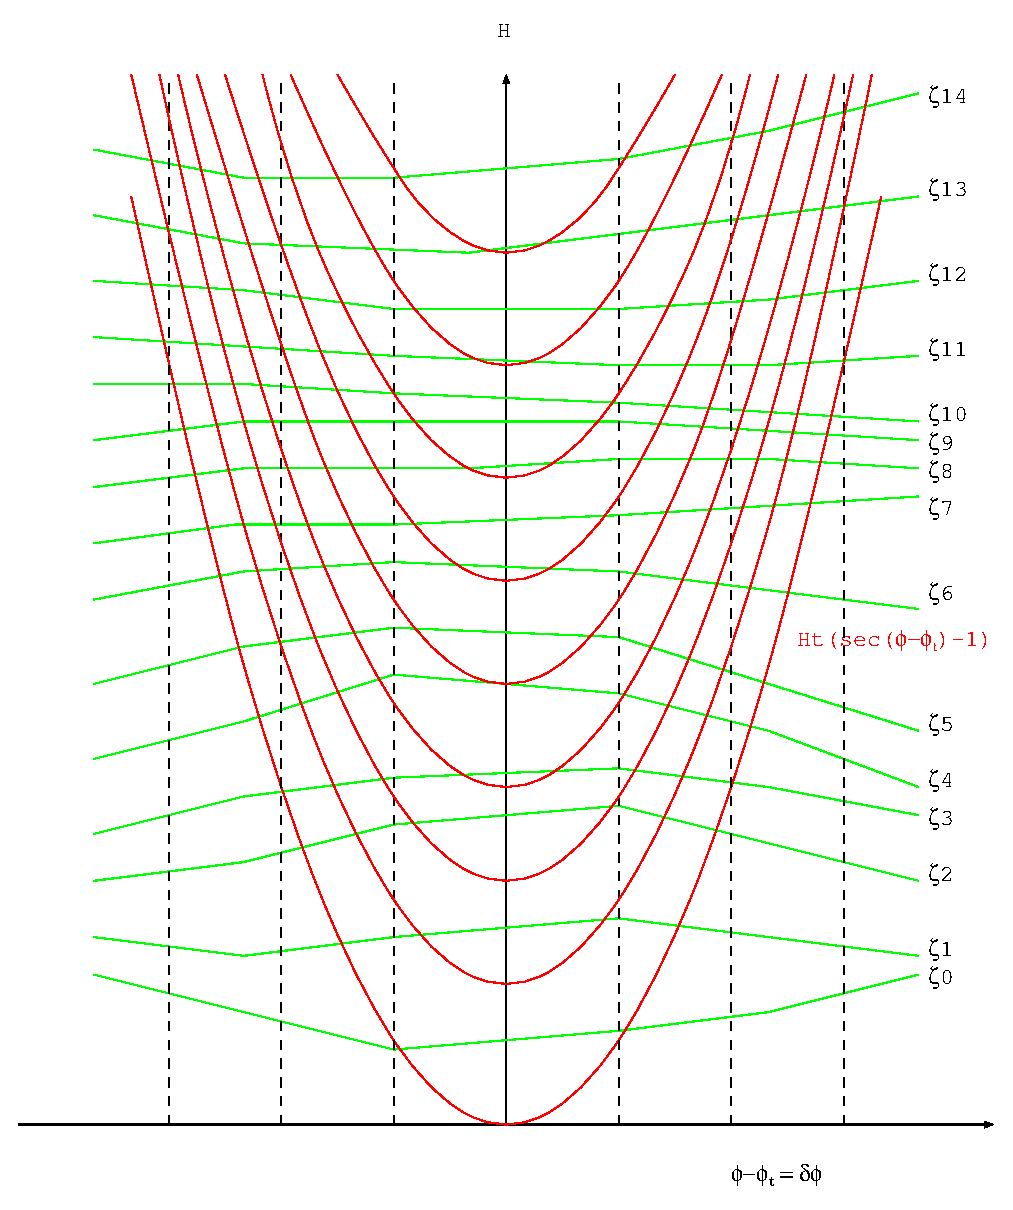
\includegraphics[width=2.25in,height=2.8125in]{wvs-048-grid2}}\\

\end{multicols}

\end{frame}
%
% -----------------------------------------------------------------------------
%
\newframe{SLAbs preparation}

SLAbs (Single Line Absorption) preparation consists of filling the structures
allocated by {\tt AllocateSlabs} with values that depend upon the spectroscopic
parameters for each relevant line, and the temperature and pressure at the
points along the line of sight computed by the Metrics calculations, but not
frequency.  This is ultimately done either by {\tt Slabs\_Prep} or {\tt
Slabs\_Prep\_dT}, depending upon whether temperature derivatives are
requested.  The computed quantities are
\begin{itemize}
\item $\nu_{0_s}$, the pressure- and doppler-shifted line center,
\item $x_1$, the Doppler half-width (MHz),
\item $y$, collision width / Doppler half-width,
\item $y_i$, interference contribution,
\item {\tt Slabs1}, frequency-independent part of {\tt Slabs},
\item $\frac{\text{d {\tt Slabs1}}}{\text{d} \nu_0}$,
\item $\frac{\text{d}\nu_{0_s}}{\text{d}T}$, $\frac{\text{d}x_1}{\text{d}T}$,
$\frac{\text{d}y}{\text{d}T}$, $\frac{\text{d}y_i}{\text{d}T}$,  and
$\frac{\text{d}{\text{\tt Slabs1}}}{\text{d}T}$ if temperature derivatives are
requested.
\end{itemize}

\end{frame}
%
% -----------------------------------------------------------------------------
%
\newframe{Frequency loop --- overview}

The frequency loop does the radiative transfer for each requested frequency. 
Frequencies are either from the pointing frequency grid (for the LBL
frequency-averaging case), or the channel centers (for monochromatic or PFA
calculations). The steps for each frequency are
\small
\begin{enumerate}
\itemsep 0pt
\item Interpolate mixing ratios from {\tt Grids\_T} to the line-of-sight path
giving $f^k_i$, for species (extinction) that depend upon frequency.
\item Evaluate $\beta^k_i$ and $\alpha_i$ for each species $k$ and each point
$i$ on the coarse path, and $\Delta\delta_{i \rightarrow i-1}$ for each layer
using a rectangular quadrature formula.
\item Call {\tt Path\_Contrib} to determine where GL is needed, using
$\Delta\tau_i$.
\item Where GL is not needed, replace $\Delta\delta_{i \rightarrow i-1}$ by a
trapezoidal estimate.
\item Evaluate $\beta^k_i$ and $\alpha_i$ for GL, and $\Delta\delta_{i \rightarrow i-1}$
using GL, where necessary.
\item Compute $\tau_i = \exp\left(-\sum_{j=2}^i \Delta\delta_{j \rightarrow
j-1}\right) \approx \exp \left( -\int_{\zeta_1}^{\zeta_i} \alpha(\zeta) \,
\text{d} \zeta \right)$.
\item Compute radiance $I = \sum_{i \in \text{layers}} \Delta B_i \tau_i$,
where $B_i = \frac{h \nu}{k \left(\exp\left(\frac{h \nu}{k
T_i}\right)-1\right)}$ is the Planck function.
\item Compute derivatives $\frac{\partial I}{\partial T_i}$ and $\frac{\partial
I}{\partial f^k_i}$ ($f^k_i$ is mixing ratio for $k^\text{th}$ species).
\end{enumerate}

\end{frame}
%
% -----------------------------------------------------------------------------
%
\newframe{Frequency loop --- $\beta$ and $\alpha$}

For each frequency and species, $\beta^k_i$ is computed using a method that
depends upon whether the calculation is LBL or PFA, scalar or polarized, or
cloudy.

\begin{itemize}
\item {\tt Get\_Beta\_Path} for scalar LBL
\item {\tt Get\_Beta\_Path\_PFA} for scalar PFA
\item {\tt Get\_Beta\_Path\_Polarized} for Polarized (which can't be PFA)
\item {\tt Get\_Beta\_Path\_Cloud} for clouds (also not PFA)
\end{itemize}

$\alpha_i = \sum_{k \in \text{species}} f^k_i \beta^k_i$, where $f^k_i$ is the
mixing ratio of the $k^{\text{th}}$ species at the $i^{\text{th}}$ point along
the line of sight.  For GL calculations, $\alpha_{ij} = \sum_{k \in
\text{species}} f^k_{ij} \beta^k_{ij}$, where $j$ indexes the GL point in the
$i^{\text{th}}$ layer.

\end{frame}
%
% -----------------------------------------------------------------------------
%
\newframe{Frequency loop --- $\Delta\delta_{i \rightarrow i-1}$ and $\tau_i$}

\small
The incremental optical depth $\Delta\delta_{i \rightarrow i-1} =
\int_{s_i}^{s_{i-1}} \alpha_i \text{d} s$.  The contribution from the $k^\text{th}$ species
is $\Delta\delta^k_{i \rightarrow i-1} =
\int_{s_i}^{s_{i-1}} f^k_i(s) \beta^k_i \text{d} s$.

Where GL is needed, these are computed in $\zeta$ coordinates, \emph{viz.}
$\Delta\delta_{i \rightarrow i-1}
\!\approx\! \sum_{j=1}^{N_{\text{GL}}} \omega_j \left(\alpha
\frac{\text{d}s}{\text{d}h} \frac{\text{d}h}{\text{d}\zeta} \right)_{ij}
\Delta\zeta $
%= \int_{\zeta_i}^{\zeta_{i-1}} \alpha_{ij} \frac{\text{d}s}{\text{d}h}
%\frac{\text{d}h}{\text{d}\zeta} \text{d} \zeta $
and
$\Delta\delta^k_{i \rightarrow i-1}
\!\approx\! \sum_{j=1}^{N_{\text{GL}}} \omega_j \left( f^k \beta^k
\frac{\text{d}s}{\text{d}h} \frac{\text{d}h}{\text{d}\zeta} \right)_{ij}
\Delta\zeta $.\\
%= \int_{\zeta_i}^{\zeta_{i-1}} f^k_{ij} \beta^k_{ij} \frac{\text{d}s}{\text{d}h}
%\frac{\text{d}h}{\text{d}\zeta} \text{d} \zeta$.\\
$s = \sqrt{h^2-h^2_t}$, so
$\frac{\text{d}s}{\text{d}h} = \frac{h}{\sqrt{h^2-h_t^2}}$, which is singular
at the tangent point $h = h_t$; this is partially canceled using the
rectangular estimate:\\
$\int_{\zeta_i}^{\zeta_{i-1}} G(\zeta) \frac{\text{d}s}{\text{d}h}
\frac{\text{d}h}{\text{d}\zeta} \text{d} \zeta =
G(\zeta_i) \int_{\zeta_i}^{\zeta_{i-1}} \frac{\text{d}s}{\text{d}h}
\frac{\text{d}h}{\text{d}\zeta} \text{d} \zeta +
\int_{\zeta_i}^{\zeta_{i-1}} [G(\zeta)-G(\zeta_i) \frac{\text{d}s}{\text{d}h}
\frac{\text{d}h}{\text{d}\zeta} \text{d} \zeta$.\\
The first integral on the right is just $\Delta s_{i \rightarrow i-1}$, so the
first term on the right is the rectangular estimate.  $G(\zeta)-G(\zeta_i) = 0$
for $\zeta = \zeta_i$, which cancels the singularity in
$\frac{\text{d}s}{\text{d}h}$ at the tangent point if $\zeta_i = \zeta_t$.

$\tau_i = \exp \left( - \sum_{j=2}^i \Delta\delta_{i \rightarrow i-1}
\right)$.  The running sum of $\Delta \delta_{i \rightarrow i-1}$ is only
taken until it exceeds $\ln \Omega$, where $\Omega$ is the largest
floating-point number, after which $\exp$ underflows, so $\tau_i = 0$
thereafter.

\end{frame}
%
% -----------------------------------------------------------------------------
%
\newframe{Frequency loop --- Derivatives}

$\frac{\partial I}{\partial f^k_i}$ is computed by {\tt DRad\_Tran\_df} from
the {\tt Rad\_Tran} module.  This is a fairly straight-forward computation. 
The derivatives are first evaluated using rectangular quadrature (integral with
respect to d$s$ of derivative w.r.t.\ mixing ratio).  Then where the radiance
path integration needed GL improvement, the derivatives are improved using GL. 
Then the refractive correction is applied.  Finally these individual integrals
are added up using Equations (10.7-9) from the ATBD using {\tt Dscrt\_dx} from
the {\tt Scrt\_dn\_m} module.  Notice that for mixing ratio derivatives
$\frac{\partial \Delta B_i}{\partial f^k_i}$ is zero.

$\frac{\partial I}{\partial T_i}$ is computed by {\tt DRad\_Tran\_dT}.  This is
similar in broad outline to {\tt DRad\_Tran\_df} but is significantly
complicated by the need to take the derivatives of hydrostatic equilibrium
w.r.t.\ temperature.  At the end the individual integrals are added up using
{\tt Dscrt\_dT}.  $\frac{\partial \Delta B_i}{\partial T_i}$ is not zero.

\end{frame}
%
% -----------------------------------------------------------------------------
%
\newframe{Pointing loop --- Frequency averaging}

If a configuration requests frequency averaging, has both LBL and PFA $\beta$'s,
and requests derivatives, some preliminary work on frequency averaging is done
by the internal subroutines {\tt Frequency\_Avg\_Rad\_Path} and {\tt
Frequency\_Average\_Derivatives}, which in turn uses {\tt
Fre\-quen\-cy\_\-Average\_Derivative}.

Then the internal subroutine {\tt Frequency\_Average} is used either to average
using the filter shapes, or just to store the result for monochromatic runs.
{\tt Fre\-quency\_Average} uses {\tt SCRT\_PFA} from the {\tt Scrt\_dn\_m}
module to combine $\tau_i$ for LBL and PFA molecules.

{\tt Fre\-quen\-cy\_\-Average\_Derivative} and {\tt Frequency\_Average} use the
subroutines {\tt Freq\_Avg} and {\tt Freq\_Avg\_DACS} from the {\tt
Freq\_Avg\_m} module.

\end{frame}
%
% -----------------------------------------------------------------------------
%
\newframe{Pointing loop --- Frequency averaging (cont.)}

The subroutine {\tt Freq\_Avg} first uses {\tt Freq\_Avg\_Setup} to find the
position in the frequency grid of the minimum and maximum frequency in the
filter shape table.

Then it uses {\tt Freq\_Avg\_Avg} to fit the radiances or derivatives with a
spline and then integrate the spline using Simpson's rule or the Newton-Cotes
3/8 rule.

The subroutine {\tt Freq\_Avg\_DACS} uses the Math77 subroutine {\tt DTCST} to
convolve DACS radiances or derivatives with the filter, using a cosine-sine
transform.

\end{frame}
%
% -----------------------------------------------------------------------------
%
\newframe{Pointing loop --- PFA}

The frequency loop is run separately, first for LBL species (if any) and then
for PFA species (if any). If there are any PFA species, the radiances from LBL
species are separately frequency averaged at every point on the path.

PFA $\beta^k_i$ is obtained by interpolation in PFA tables instead of
spectroscopic modeling.

$\tau_i$ for PFA is multiplied by the frequency-averaged radiance from the LBL
calculation, and the product summed to give combined LBL and PFA radiance for
the channel.  See wvs-028 and its references.

Temperature derivatives are computed as if they were mixing-ratio derivatives,
to avoid including the Planck function twice.

LBL and PFA derivatives are simply added during the frequency-averaging step.

\end{frame}
%
% -----------------------------------------------------------------------------
%
\newframe{Sideband loop --- Antenna convolution}

The internal subroutine {\tt Convolution} either convolves the radiances and
derivatives from all the pointings with the antenna pattern, or just
interpolates them to PTan.

First, it makes sure the pointing angles are strictly increasing, and patches
them in an ad-hoc way if not.

Then it works out which antenna pattern to use, and applies the elevation
offset.

Then it uses {\tt FOV\_Convolve\_Setup} from the
{\tt FOV\_Convolve\_m} module to fill the {\tt Convolve\_Support} structure with
data that depend only on pointing angles.

\end{frame}
%
% -----------------------------------------------------------------------------
%
\newframe{Sideband loop --- Antenna convolution (cont.)}

\small
Using the {\tt Convolve\_Support} structure, the radiances are convolved using
the following subroutines from the {\tt Convolve\_All\_m} module:
\begin{itemize}
\item {\tt Convolve\_Radiance} for radiances.
\item {\tt Convolve\_Temperature\_Deriv} for temperature derivatives.  The
temperature derivative also includes hydrostatic contributions that model the
effect of a temperature change on the antenna pattern that is remapped onto
$\zeta$ coordinates.
\item {\tt Convolve\_Other\_Deriv} for mixing-ratio or spectroscopy-parameter.
derivatives
\end{itemize}

The subroutine {\tt Convolve\_Radiance} uses the subroutine {\tt
FOV\_Con\-volve\_\-1d} from the module {\tt FOV\_Convolve\_m}.  The subroutine
{\tt Con\-volve\_\-Tem\-perature\_Deriv} uses the subroutine {\tt
FOV\_Con\-volve\_\-Temp\_Derivs}.  The subroutine {\tt Convolve\_Other\_Deriv}
uses the subroutine {\tt FOV\_Convolve\_2d}.

The subroutines in the module {\tt FOV\_Convolve\_m} use the Math77 subroutines
{\tt DTCST} to compute a cosine transform, and {\tt DRFT1} to compute a full
FFT.

\end{frame}
%
% -----------------------------------------------------------------------------
%
\newframe{Sideband loop --- No antenna convolution}

If antenna convolution is not requested, the subroutine {\tt
Inter\-po\-late\_\-Array\_Setup} from the module {\tt MLSNumerics} is used. 
Then the following subroutines from the module {\tt Convolve\_All\_m} are used:
\begin{itemize}
\item {\tt Interpolate\_Radiance} to interpolate radiance
\item {\tt Interpolate\_Temperature\_Deriv} to interpolate temperature
derivatives
\item {\tt Interpolate\_Other\_Deriv} to interpolate mixing-ratio and
spectroscopy-parameter derivatives
\end{itemize}

\end{frame}
%
% -----------------------------------------------------------------------------
%
\newframe{Sideband loop --- Cleaning up}

After antenna convolution or interpolation to PTan, the subroutines {\tt
ScanAverage\_1d} and {\tt ScanAverage\_2d} from the module {\tt ScanAverage\_m}
are used to average the radiances and derivatives, respectively, from the
pointing angles to the MIF angles, taking motion during the MIF into account.

The subroutine {\tt Interpolate\_Values} is used to interpolate radiances and
derivatives to eight-point grids GL between each pair of values from the {\tt
MIF\_Times} grid.  Those interpolated values are then integrated to the {\tt
MIF\_Times} grid using an eighth-order Gauss-Legendre quadrature.

Finally, some arrays explicitly allocated in {\tt FullForwardModelAuto} are
deallocated, and some debug printing is done if requested.

\end{frame}
%
% -----------------------------------------------------------------------------
%
\newframe{References (1)}

\small
The primary reference is the Full Forward Model ATBD, JPL D-18130.

Many of the modules have embedded \LaTeX-isms, and can be turned into \LaTeX\
files from which nice listings with typeset mathematics can be produced by using
my $\sim${\tt vsnyder/progs/f90tex} program.

Several of my memos (in $\sim${\tt vsnyder/mls/doc/}) might be helpful:

\begin{itemize}
\item wvs-017: Pre-frequency averaging
\item wvs-018: Temperature derivatives
\item wvs-019: Betas, {\tt slabs\_sw\_m}
\item wvs-022: Spectroscopy derivatives
\item wvs-024: PFA derivatives
\item wvs-025: New frequency averaging scheme for use with PFA
\item wvs-026: Simplifying assumption to combine line-by-line and PFA
\item wvs-027: Revised method to combine line-by-line and PFA
\item wvs-028: Summary of line-by-line and PFA radiance and derivatives
\end{itemize}
\end{frame}
%
% -----------------------------------------------------------------------------
%
\newframe{References (2)}

\begin{itemize}
\item wvs-029: Refractive correction for $\phi$
\item wvs-033: Path integrations [a proposal, not a description]
\item wvs-037: Updated non-GL correction in forward model
\item wvs-038: Modification to {\tt metrics\_m}
\item wvs-039: Calculating $H_m$ in modification to {\tt metrics\_m}
\item wvs-040: Calculating $\phi$ for $\zeta_{\text{max}}$ [should be
$\zeta_{\text{min}}$]
\item wvs-041: Maximum [should be Minimum] $\zeta$
\item wvs-042: $H$--$\phi$ iteration in {\tt metrics}
\item wvs-043: Inverting the $\phi$ refractive correction
\item wvs-044: What to do in {\tt metrics\_m}
\item wvs-046: Interesting result concerning $\zeta_{\text{min}}$
\item wvs-047: Revised metrics plan
\item wvs-048: Different solution for $\phi$--$H$ calculation in {\tt metrics\_m}
\item wvs-053: Alternative minimum $\zeta$ calculation
\end{itemize}
\end{frame}
%
% -----------------------------------------------------------------------------
%
\newframe{References (3)}

\begin{itemize}
\item wvs-056: Refractive correction
\item wvs-059: Another look at metrics [turned out to be a bad idea]
\item wvs-060: Trouble with GL correction in the forward model
\item wvs-061: Trouble with path length in the forward model
\end{itemize}

\end{frame}
%
% ----------------------------------------------------------------------------
%
\end{document}

%%% Local Variables: 
%%% mode: latex
%%% TeX-master: t
%%% End: 

% $Log$
% Revision 1.2  2019/05/23 00:26:28  vsnyder
% Convert to beamer class
%
% Revision 1.1  2008/06/11 20:14:54  vsnyder
% Initial commit
%
% Revision 1.1  2008/06/11 20:14:54  vsnyder
% Initial commit
%
% Revision 1.7  2001/06/16 00:57:56  vsnyder
% More stuff about least-squares, some clean-up
%
% $Id$
